\documentclass{beamer}
\usepackage{textcomp}
\usepackage[utf8]{inputenc}
\usepackage{adjustbox}

\setbeamerfont{footnote}{size=\tiny}
\usetheme{Boadilla}
\usecolortheme{seagull}

\usepackage{fancyvrb}
\newenvironment{myverb}{% Verbatim shrinked
 \VerbatimEnvironment
 \begin{adjustbox}{max width=\linewidth}
 \begin{BVerbatim}
  }{
  \end{BVerbatim}
 \end{adjustbox}
}
\title{ChIP-Seq technical pipeline}
\author{\href{mailto:os@jetbrains.com}{Oleg Shpynov}}
\institute{JetBrains Biolabs}

\date{\today}

\begin{document}

\begin{frame}
  \titlepage
\end{frame}

\begin{frame}{Agenda}
\begin{itemize}
	\item Reads QC
	\item Alignment
	\item Peaks calling
	\item Differential peak calling
	\item Pipeline sketch
\end{itemize}
\end{frame}

\begin{frame}{Reads QC}

\includegraphics[width=\linewidth]{ngstoolkit.png}\\
Only a few standalone tools for QC of NGS data are publicly available other than commercial softwares supplied with the sequencing machines, which are not sufficiently optimal.
\end{frame}

\begin{frame}
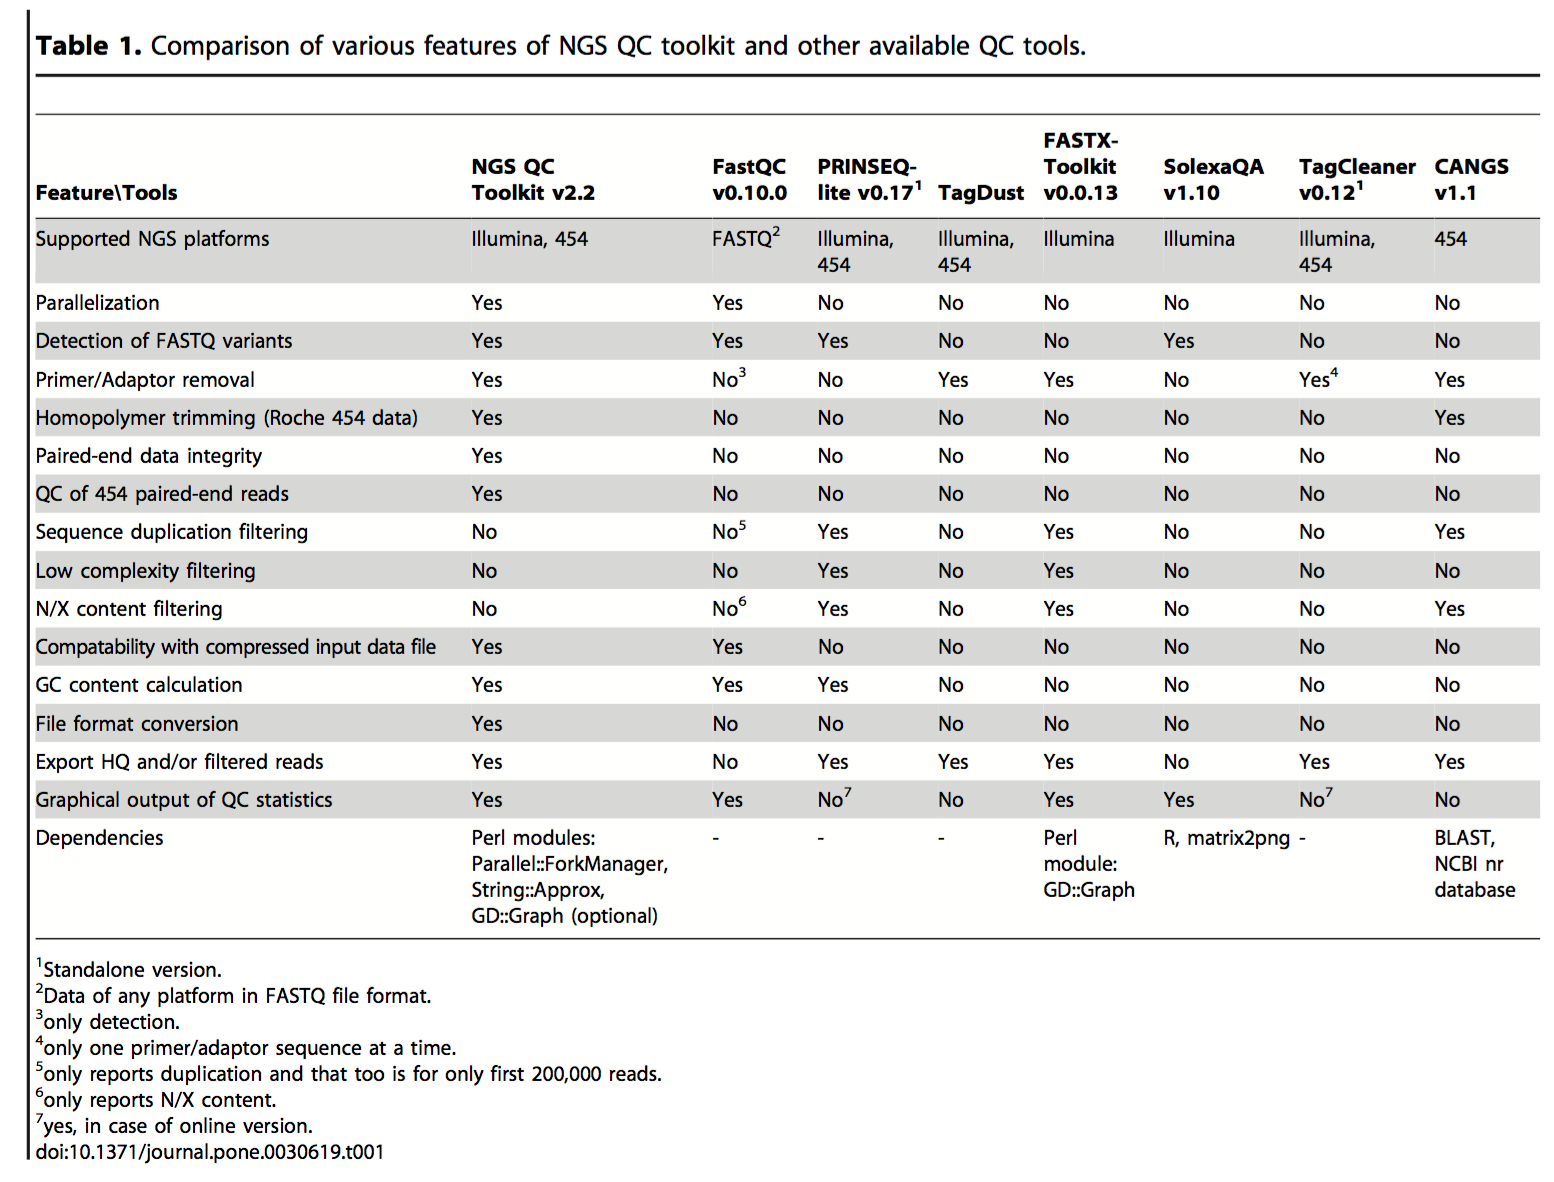
\includegraphics[width=\linewidth]{readsqc.png}
\end{frame}

\begin{frame}{FastQC}
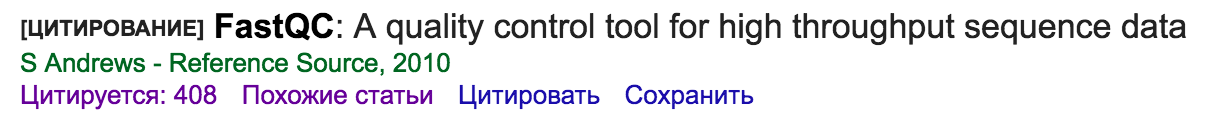
\includegraphics[width=\linewidth]{fastqc.png}
\end{frame}

\begin{frame}
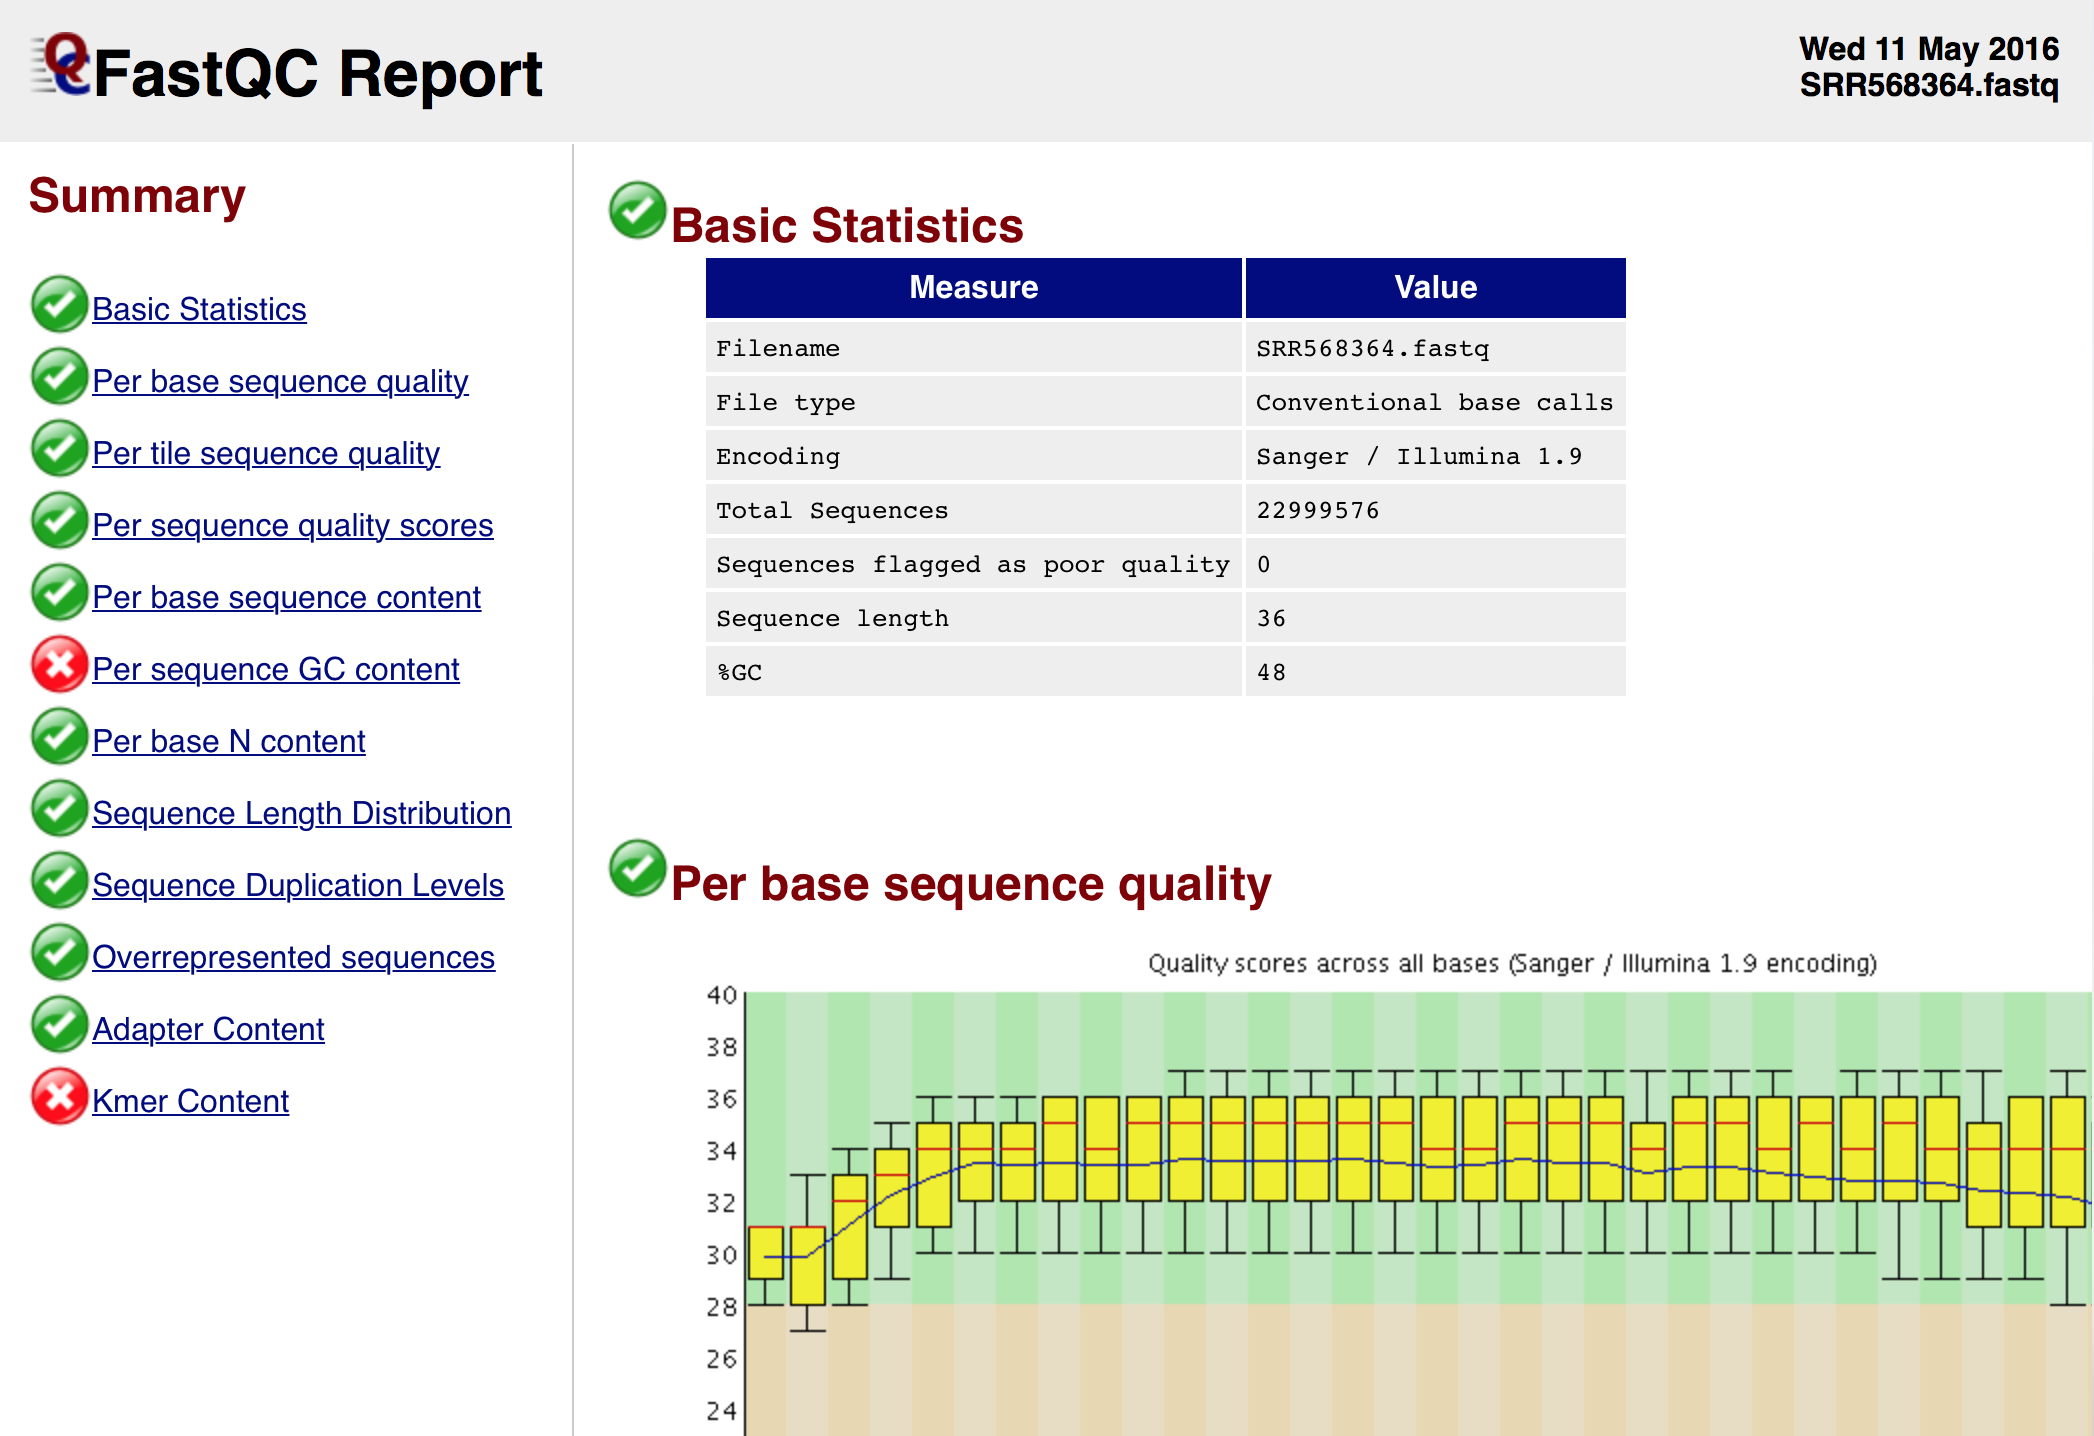
\includegraphics[width=\linewidth]{fastqcrep.png}
\end{frame}


\begin{frame}{Alignment}
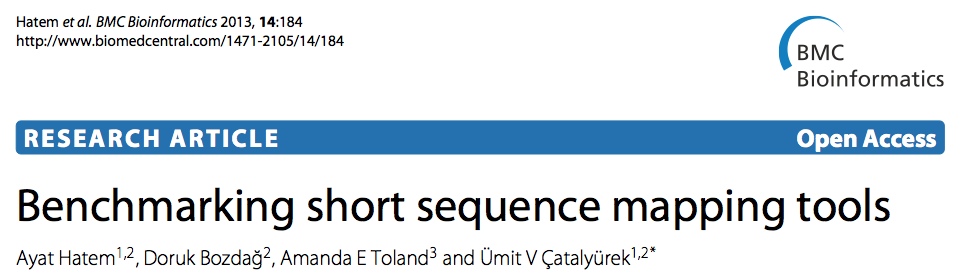
\includegraphics[width=\linewidth]{mappaper.png}
\end{frame}

\begin{frame}{Alignment}
\begin{itemize}
\item SNPs: GSNAP’s filtered output helped in detecting the largest number of SNPs.
\item The evaluation of Bowtie, Bowtie2, BWA, mrsFAST, and Novoalign show their ability to correctly map the reads.
\item Genome: further investigations are required to understand the different properties of the genomes and their effect on the different mapping techniques.
\item Mismatches: Bowtie output mappings are more accurate than the other tools.
\item Indels: Tools like Maq and Bowtie will not map reads if there is an insertion or deletion. I have used BWA to map 75bp Illumina reads at 20x coverage to a 30Mb fungal genome with good results.\footnote{\url{https://www.biostars.org/p/97197/}}
\item In general, there is no \textbf{the-best} tool among all of the tools; each tool was \textbf{the-best} in certain conditions.
\end{itemize}
\end{frame}

\begin{frame}{Popular aligners}
BWA\\
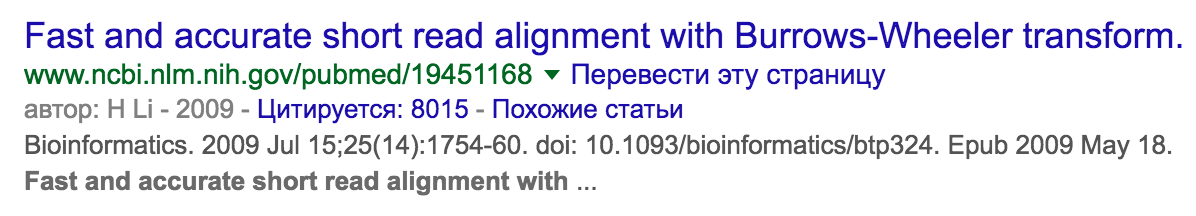
\includegraphics[width=\linewidth]{bwa.png}\\
Bowtie\\
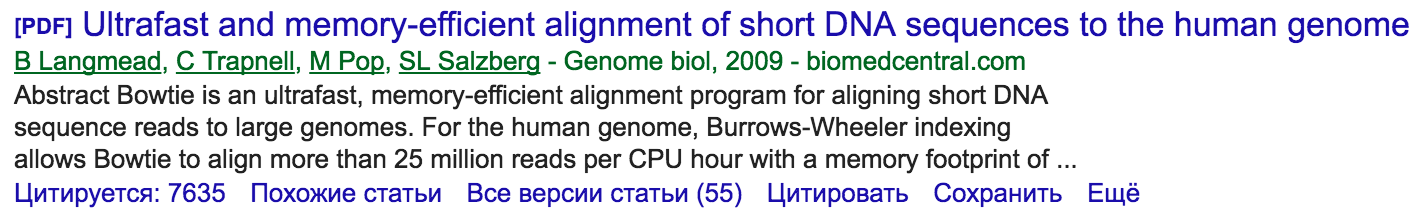
\includegraphics[width=\linewidth]{bowtie.png}\\
\end{frame}

\begin{frame}{Less popular}
MAQ\\

\includegraphics[width=\linewidth]{MAQ.png}\\
PASH\\
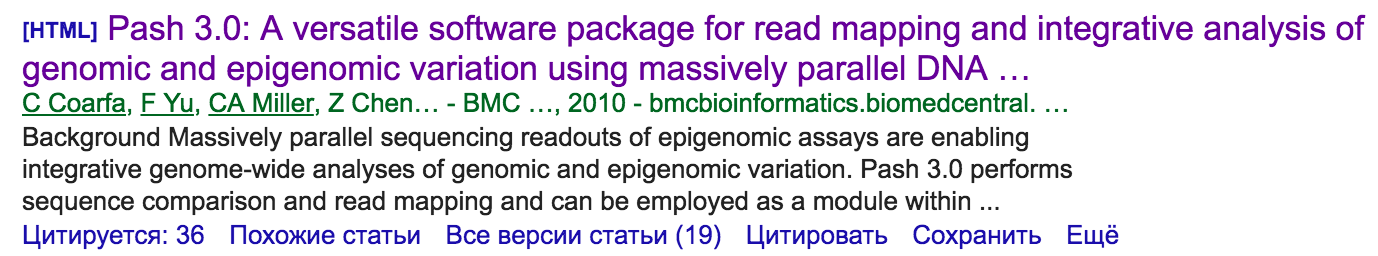
\includegraphics[width=\linewidth]{pash.png}\\
\end{frame}

\begin{frame}{Mega projects}
\begin{itemize}
\item ENCODE: MAQ\\
ChIP-seq reads were aligned to human genome build HG18 with MAQ using default parameters. All reads were truncated to 36 bases before alignment.\footnote{\url{http://www.nature.com/nature/journal/v473/n7345/abs/nature09906.html}}
\item Roadmapepigenomics: PASH\\
Sequenced data sets from the Release 9 of the Epigenome Atlas involved mapping a total of 150.21 billion sequencing reads onto hg19 assembly of the human genome using the PASH read mapper. These read mappings were used (except for RNA-seq data sets) for constructing the 111 consolidated epigenomes. Only uniquely mapping reads were retained and multiply-mapping reads were filtered out (subsampling to 30mln reads, ignoring blacklisted regions).\footnote{\url{http://www.nature.com/nature/journal/v518/n7539/full/nature14248.html}}
\end{itemize}
\end{frame}

\begin{frame}{ENCODE guideline}
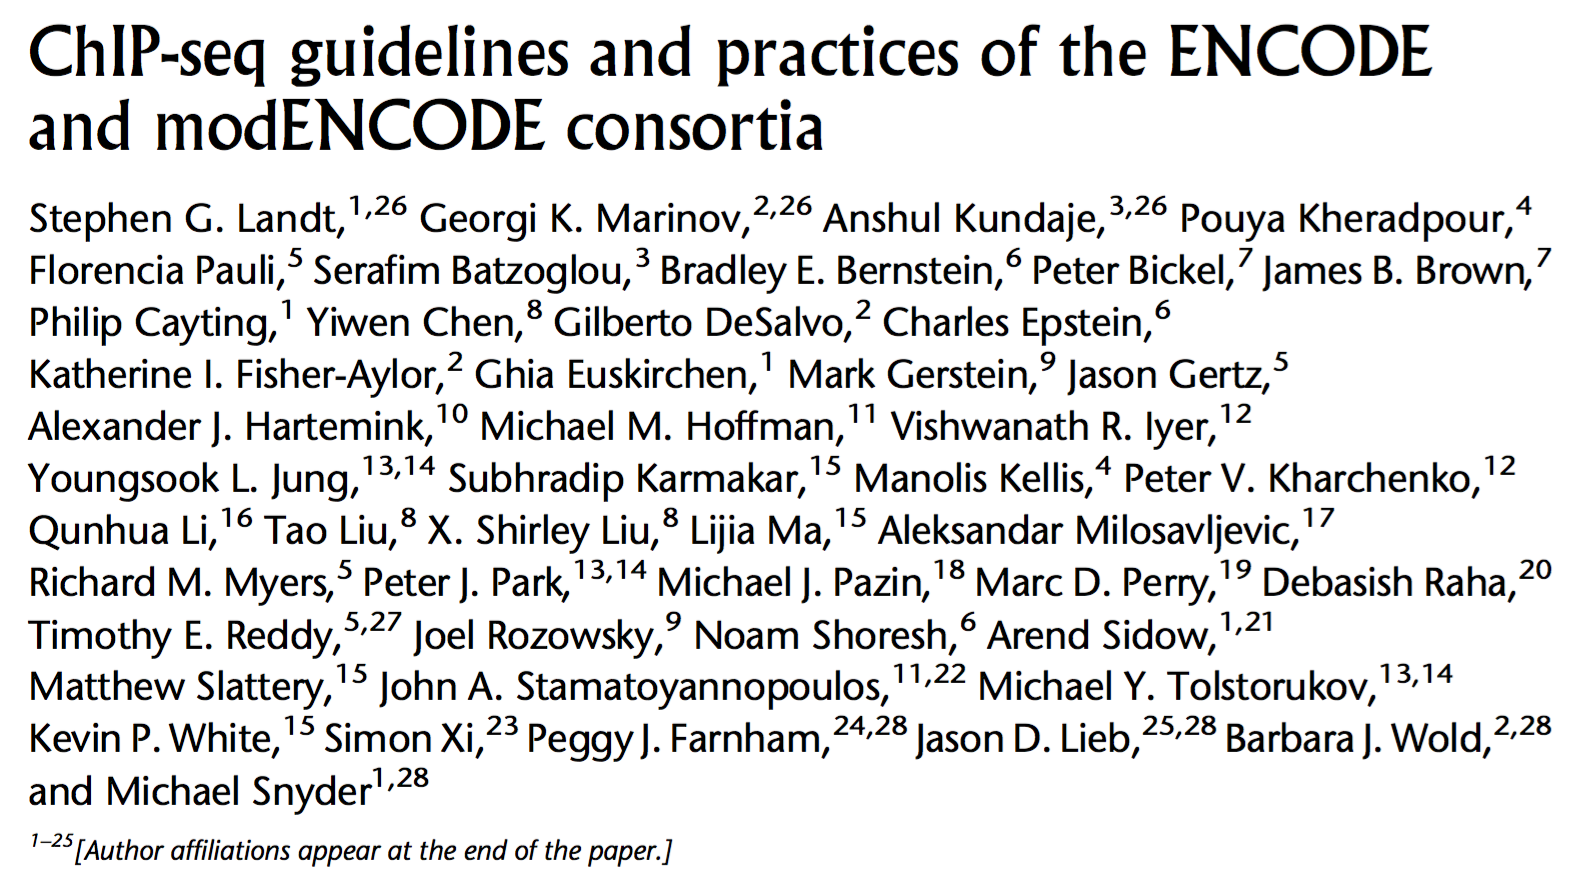
\includegraphics[width=\linewidth]{paperENCODE.png}
\end{frame}

\begin{frame}
The ENCODE and modENCODE consortia have performed more than a thousand individual ChIP-seq experiments for more than 140 different factors and histone modifications in more than 100 cell types in four different organisms.
\end{frame}

\begin{frame}
\centering{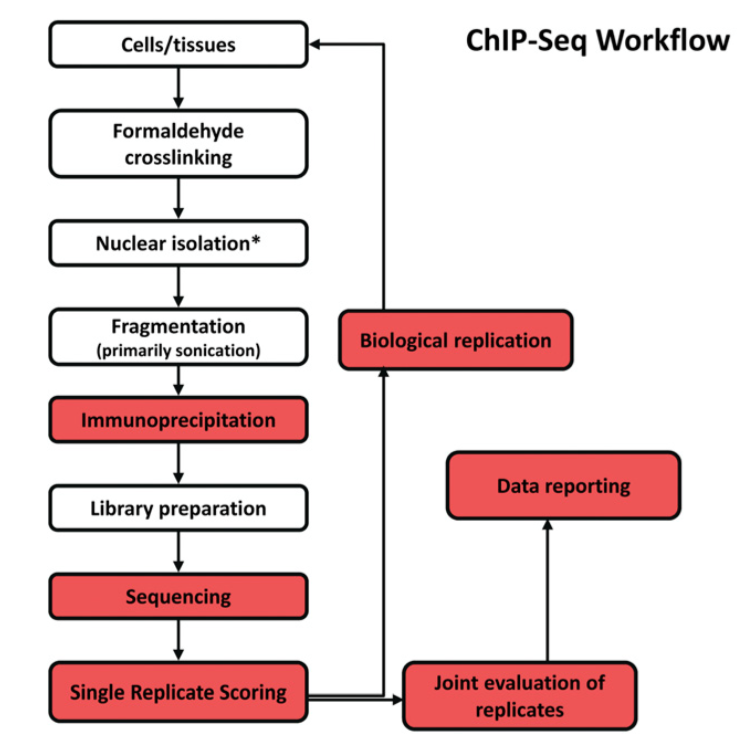
\includegraphics[height=0.8\paperheight]{ENCODE_chipseq_workflow.png}}
\end{frame}

\begin{frame}{Different sizes}
\begin{itemize}
\item \textbf{Point-source} factors and certain chromatin modifications are localized at specific positions that generate highly localized ChIP-seq signals. This class includes most sequence-specific transcription factors, their cofactors, and, with some caveats, transcription start site or enhancer-associated histone marks. These comprise the \textit{majority} of ENCODE and modENCODE determinations and are therefore the primary focus of this work.
\item \textbf{Broad-source} factors are associated with large genomic domains. Examples include certain chromatin marks (H3K9me3, H3K36me3, etc.) and chromatin proteins associated with transcriptional elongation or repression.
\item \textbf{Mixed-source} factors can bind in point-source fashion to some locations of the genome, but form broader domains of binding in others. RNA polymerase II, as well as some chromatin modifying proteins (e.g., SUZ12) behave in this way.
\end{itemize}
\end{frame}



\begin{frame}{Wet lab}
Problem: poor reactivity against the intended target and/or cross-reactivity with other DNA-associated proteins.\\
One of five criteria:
\begin{itemize}
\item factor ‘‘knockdown’’ by mutation or RNAi
\item independent ChIP experiments using antibodies against more than one epitope on a protein or against different members of the same complex
\item immunoprecipitation using epitope-tagged constructs
\item affinity enrichment followed by mass spectrometry
\item binding-site motif analysis
\end{itemize}
20\% (44 of 227) of the tested commercially available antibodies against \textbf{transcription factors} meet these characterization guidelines and also function in ChIP-seq assays.
\end{frame}

\begin{frame}{Replication, sequencing depth, library complexity}
\begin{itemize}
\item RNA polymerase II ChIP-seq experiments showed that more than two replicates did not significantly improve site discovery. Each ChIP-Seq should performed on two independent biological replicates
\item One cannot a priori set a specific target threshold for ChIP peak number or ChIP signal strength that will assure inclusion of all functional sites
\item For point-source factors in mammalian cells, a minimum of 10 million uniquely mapped reads are used by ENCODE for each biological replicate.
\item Input DNA or IgV control required - the same as the number of PCR amplification cycles, read length, etc.
\end{itemize}
\end{frame}

\begin{frame}{NFR}
Nonredundant fraction or NRF = the ratio between the number of positions in the genome that uniquely mappable reads map to and the total number of uniquely mappable reads. \\
Target is NRF $\geq$ 0.8 for 10 million uniquely mapped reads.\\
Distribution over ENCODE datasets:\\
\centering{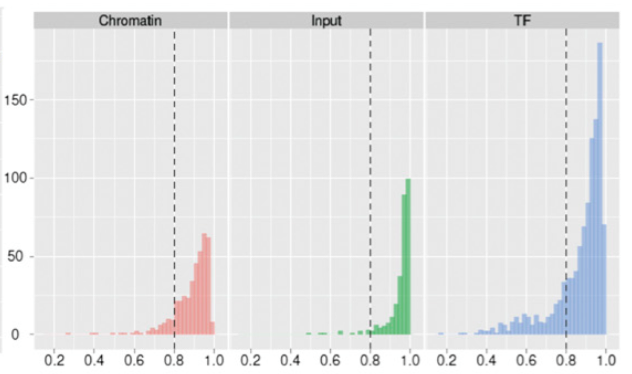
\includegraphics[height=0.5\paperheight]{nrf.png}}
\end{frame}

\begin{frame}{Peak calling}
\begin{itemize}
\item Punctate-source: several peak calling algorithms and corresponding software packages, including SPP, PeakSeq, and MACS. Too relaxed thresholds lead to a high proportion of false positives for each replicate, but subsequent replicates based analysis can strip false positives from a final joint peak determination.
\item Broad-source factors or Mixed-source: more challenging. Methods to identify such regions are emerging: ZINBA, Scripture\footnote{Originally developed for lincRNAs} and MACS2.\footnote{SICER not mentioned as of 2012}
\end{itemize}
\end{frame}

\begin{frame}{Peak calling Metrics}
\begin{itemize}
\item Successful experiments generally identify thousands to tens of thousands of peaks for most TFs. A true signal is expected to show a clear asymmetrical distribution of reads mapping to the forward and reverse strands around the midpoint (peak) of accumulated reads.
\item Visual control: inspection of mapped sequence reads using a genome browser
\item FRiP - fraction of reads in peaks. ENCODE data sets have a FRiP enrichment of 1\% - quality threshold.\footnote{ZNF274 and human RNA polymerase III have very few true binding sites and a FRiP of <1\% is obtained}
\item Strand cross-correlation: Pearson linear correlation between the Crick strand and the Watson strand, after shifting Watson by k base pairs, where k is fragment size(fragment-length cross correlation). 
\item NSC - normalized strand coefficient. The normalized ratio between the fragment-length cross-correlation peak and the background cross-correlation (normalized strand coefficient) and the ratio between the fragment- length peak and the read-length peak (relative strand correlation, RSC).\footnote{TODO: not clear enough}
\end{itemize}
\end{frame}

\begin{frame}
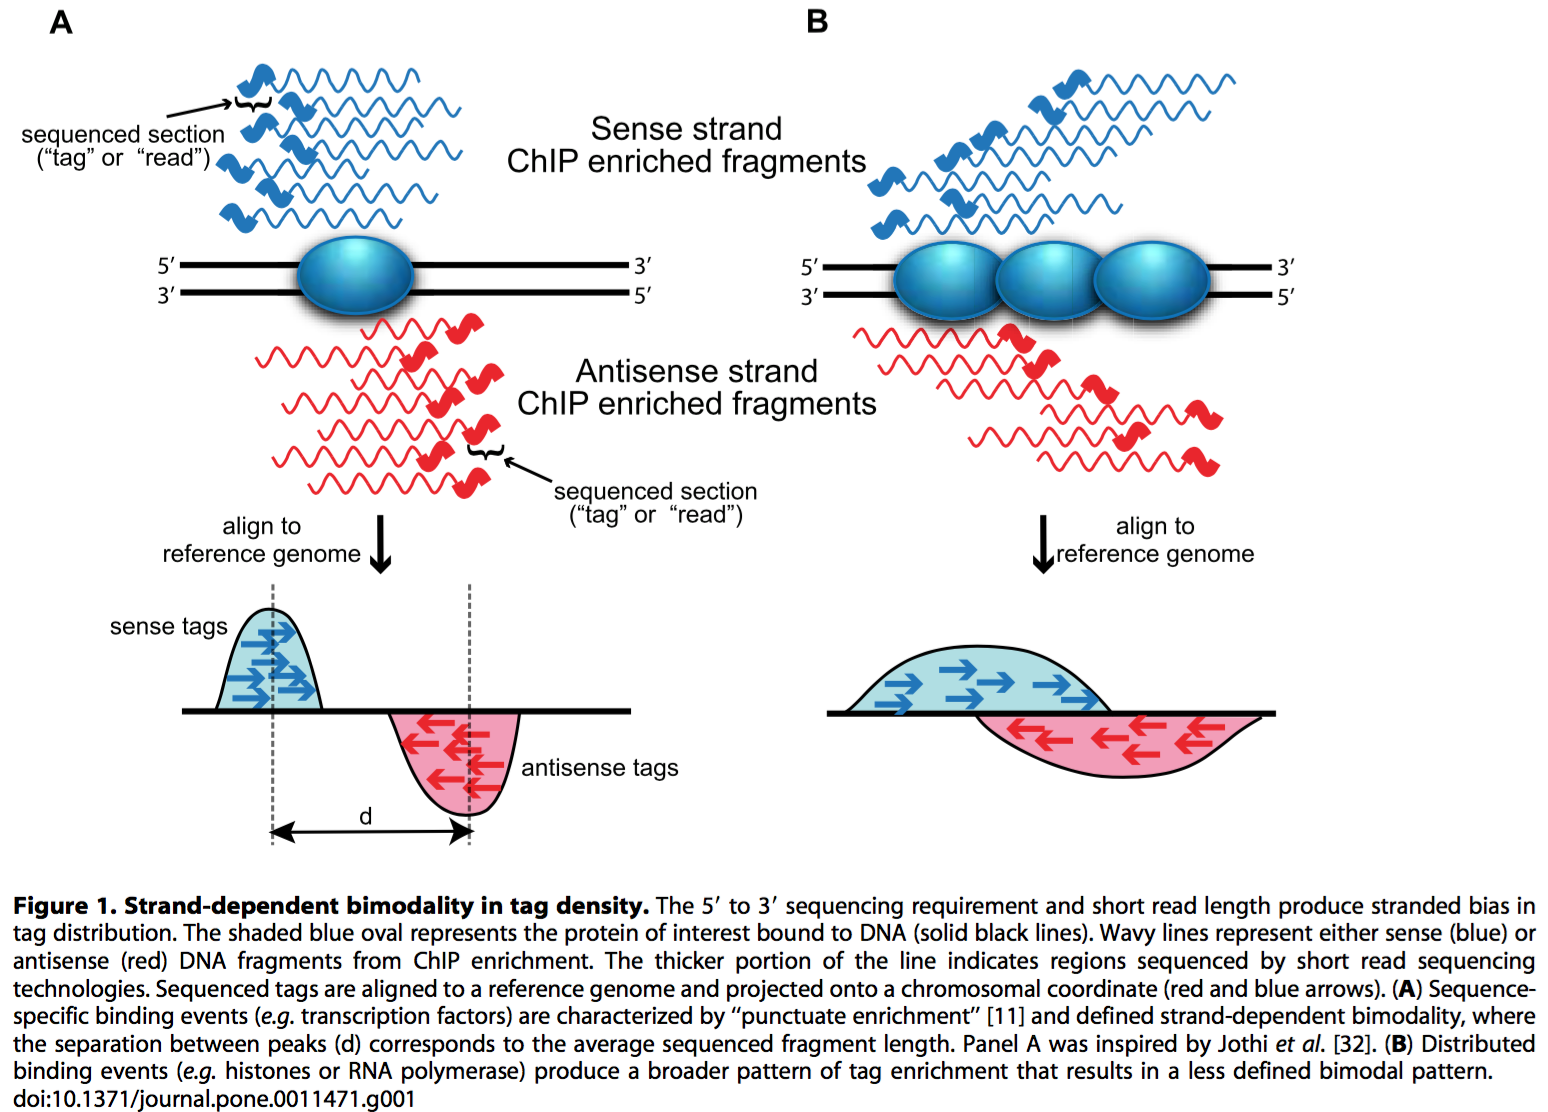
\includegraphics[width=\linewidth]{chipseq.png}\footnote{\url{http://journals.plos.org/plosone/article?id=10.1371/journal.pone.0011471}}
\end{frame}

\begin{frame}{IDR - irreproducible discovery rate}
Given a set of peak calls for a pair of replicate data sets, the peaks can be ranked based on a criterion of significance, such as the P-value, the q-value, the ChIP-to-input enrichment, or the read coverage for each peak.\\
The most significant peaks, which are likely to be genuine signals, are expected to have high consistency between replicates, whereas peaks with low significance, which are more likely to be noise, are expected to have low consistency.\\
A \textbf{major advantage} of IDR is that it can be used to establish a stable threshold for called peaks that is more consistent across laboratories, antibodies, and analysis protocols (e.g., peak callers) than are FDR measures (different for each tool).\footnote{A caution in applying IDR is that it is dominated by the weakest replicate. Additional qc is required}
\end{frame}

\begin{frame}
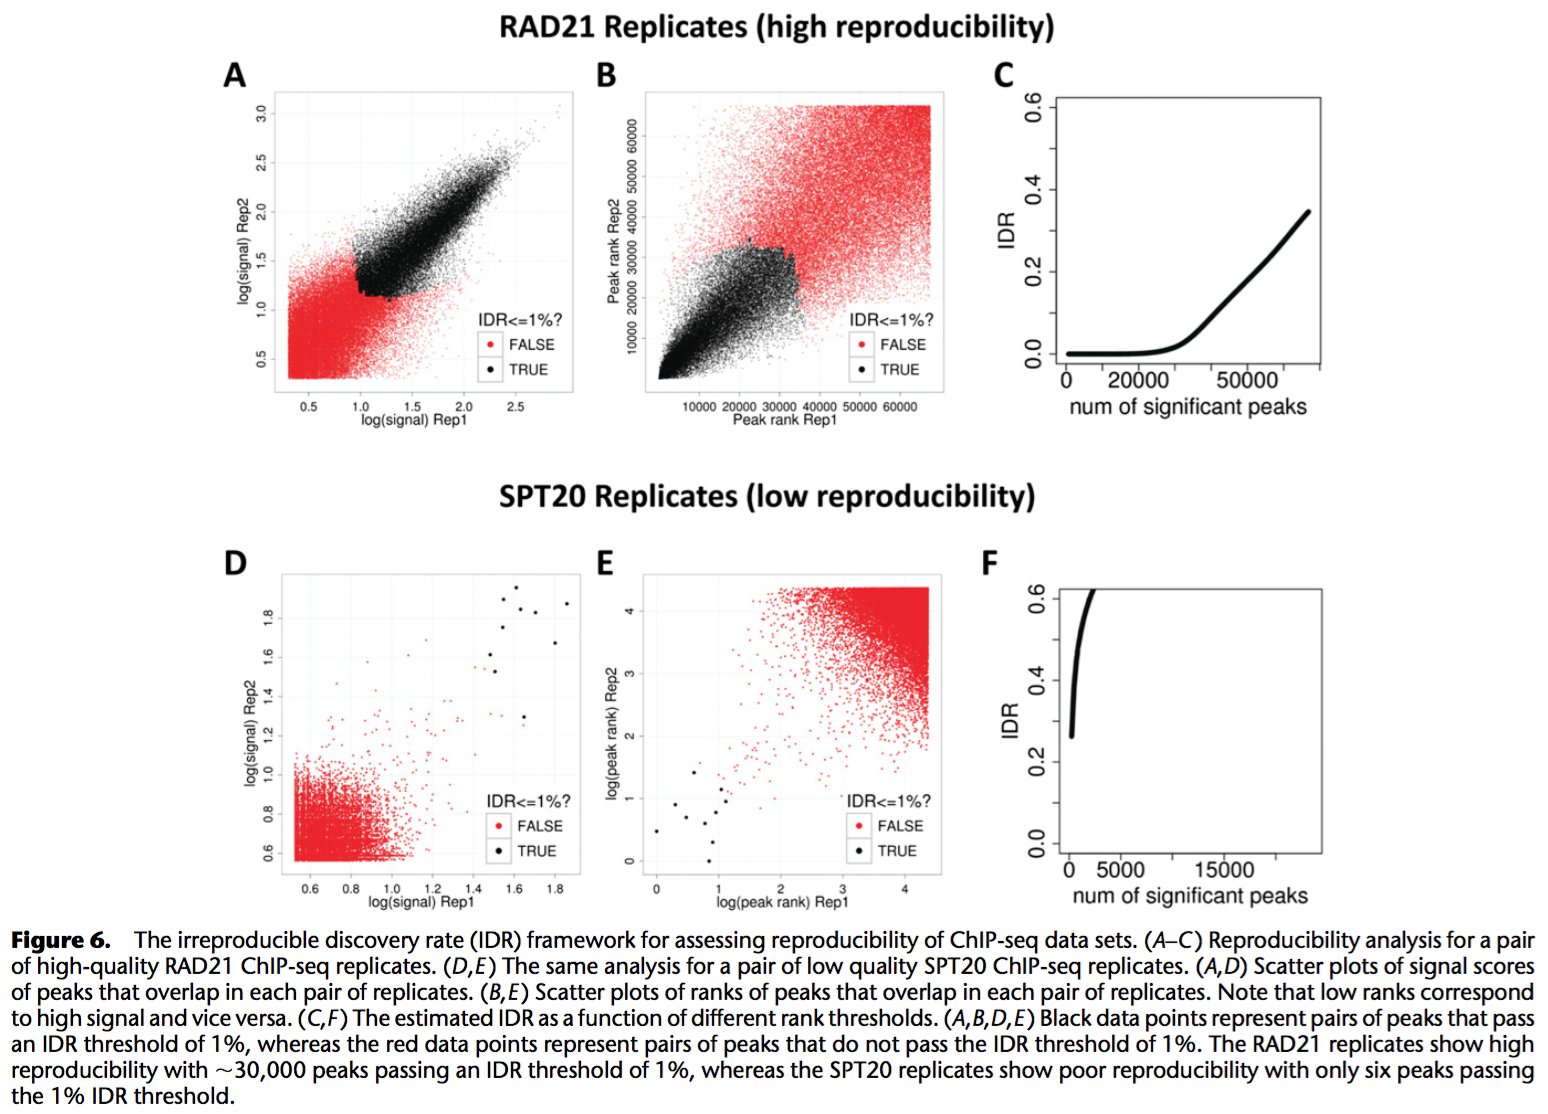
\includegraphics[width=\linewidth]{idr.png}
\end{frame}


\begin{frame}{Summary\footnote{\url{http://encodeproject.org/ENCODE/experiment_guidelines.html}}}
\begin{itemize}
\item Read depth $\geq$ 10 mln reads
\item 2 biological replicates
\item NFR\footnote{This will fail ENCODE guideline, because of new protocol}
\item FRiP
\item Strand cross-correlation
\item NSC for sharp histone modifications 
\item IDR
\end{itemize}
\end{frame}

\begin{frame}
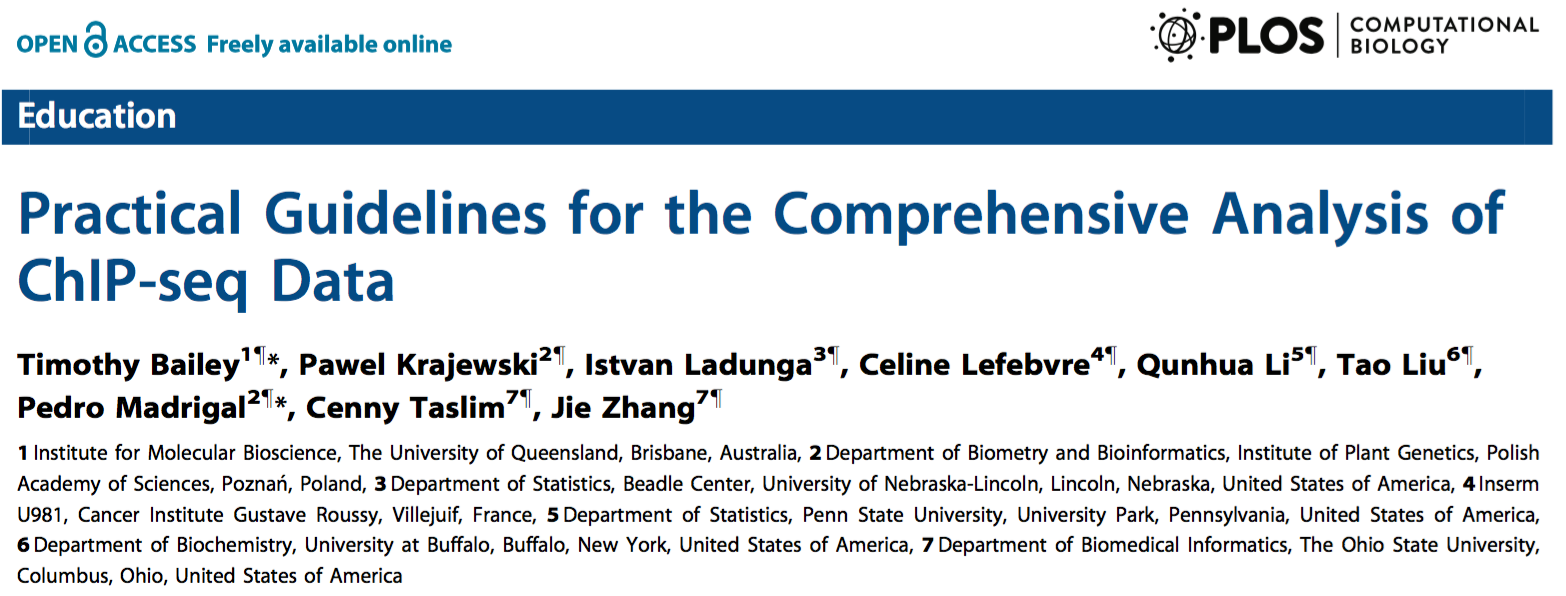
\includegraphics[width=\linewidth]{paperChipSeq.png}
\end{frame}

\begin{frame}
\centering{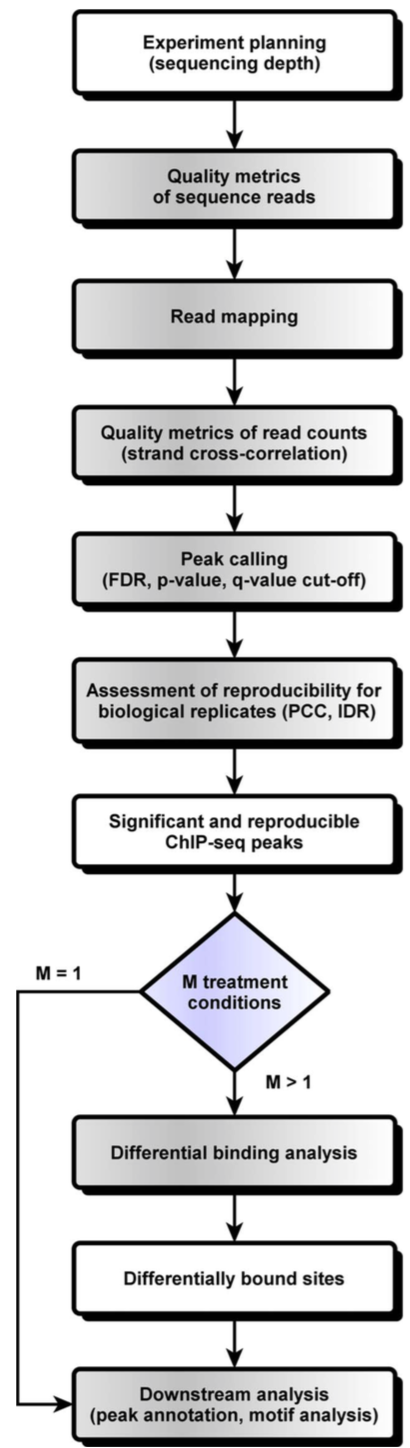
\includegraphics[height=0.9\paperheight]{chipseqworkflow.png}}
\end{frame}

\begin{frame}{Library complexity}
\begin{itemize}
\item Sufficient read depth? - saturation analysis. The peaks called should be consistent performed on increasing numbers of reads chosen at random from the actual reads (built in SPP peak caller).
\item Library complexity is a common quality measure for ChIP-seq libraries (preseq or PCR bottleneck coefficient from ENCODE tools\footnote{\url{https://code.google.com/p/phantompeakqualtools/}}).
\item NSC and RSC: very successful ChIP experiments generally have NSC $\geq$ 1.05 and RSC $\geq$ 0.8.
\item IP strength: the software CHANCE assesses IP strength by estimating and comparing the IP reads pulled down by the antibody and the background, using a method called signal extraction scaling.
\item Duplicate (identical) reads - a challenge. One can remove a certain number of duplicates to call confident peaks, and then put duplicates back to refine properties of these peaks such as peak height and boundaries.
\end{itemize}

\end{frame}
\begin{frame}{Alignment}
\begin{itemize}
\item The percentage varies between organisms, and for human, mouse, etc, above 70\% uniquely mapped reads is normal, whereas less than 50\% may be cause for concern.
\item SNR - signal-to-noise ratio. SNR can be estimated by strand cross-correlation or IP enrichment estimation using the software package CHANCE. Strand cross-correlation analysis is built into some peak callers (e.g., SPP or MACS2).
\item The reproducibility of the reads can be measured by computing the Pearson correlation coefficient (PCC) of the (mapped) read counts at each genomic position\footnote{Only position with reads are taken into account}. High quality experiments: PCC $\geq$ 0.9. (0.3 for unrelated samples).
\end{itemize}
\end{frame}

\begin{frame}{Peak calling}
\begin{itemize}
\item Punctate-source: SPP and MACS2 use cross-correlation to find the lag between reads mapped to the minus and the plus strand as the size of actual protein-DNA interacting regions. After smoothing, background models are then used to remove noise either directly from the control sample or from features of the genome sequence such as GC content or mappability.
\item Broad enriched: Several peak callers are specifically designed for predicting broad regions from ChIP-seq data, including SICER, CCAT, ZINBA, and RSEG.
\item Mixed: Some tools have options for both narrow and broad peak calling, such as SPP, MACS, ZINBA, and PeakRanger. 
\end{itemize}
\end{frame}

\begin{frame}{Summary\footnote{Additional to previous}}
\begin{itemize}
\item Unique alignment rate
\item Saturation analysis
\item IP strength
\item PCC
\end{itemize}
\end{frame}


\begin{frame}{Peak calling}
Guidelines above are better, these are old and don't cover some tools:\\
2010\\
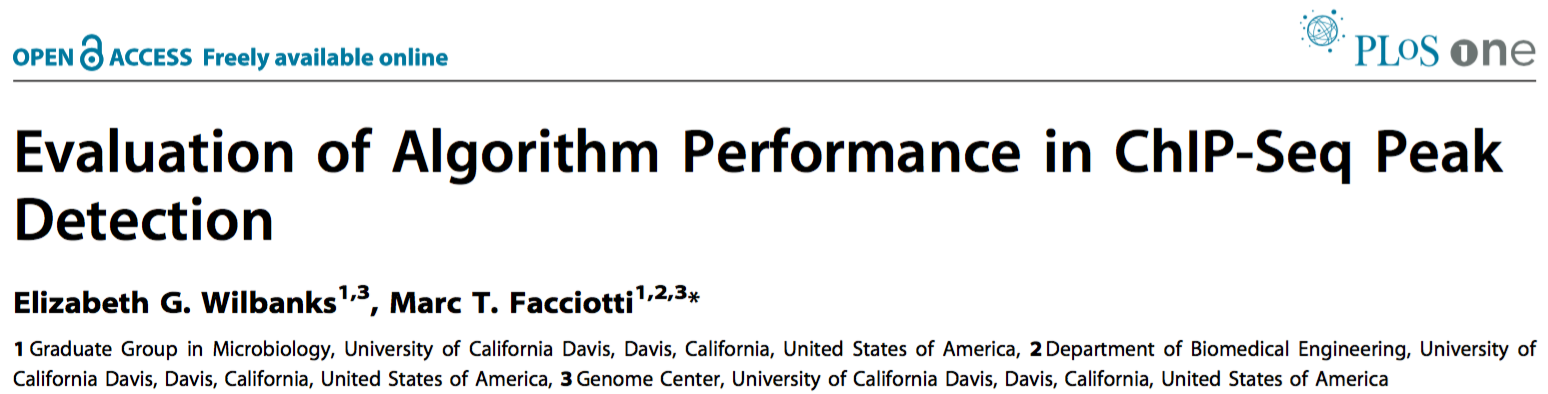
\includegraphics[width=\linewidth]{peakcalling1.png}\\
2014\\

\includegraphics[width=\linewidth]{peakcalling2.png}
\end{frame}

\begin{frame}{Popular}
MACS2\footnote{Roadmapepigenomics: Integrative analysis of 111 reference human epigenomes}\\
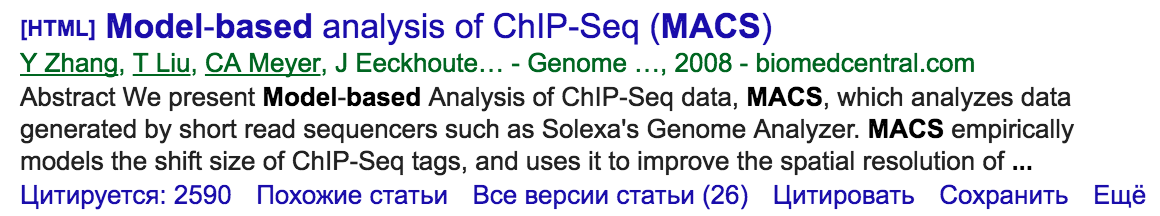
\includegraphics[width=\linewidth]{MACS2.png}\\
Scipture\\

\includegraphics[width=\linewidth]{scripture.png}\\
PeakSeq\\
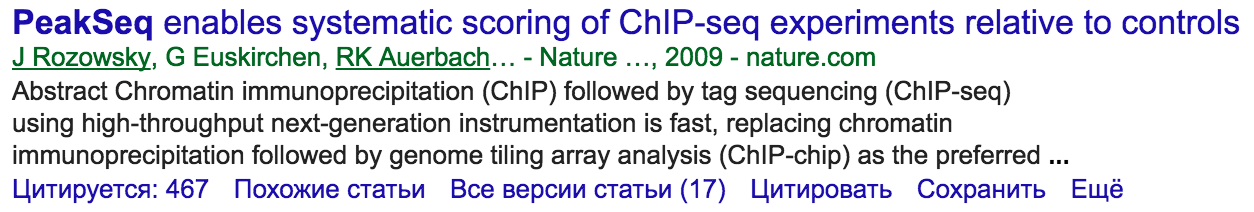
\includegraphics[width=\linewidth]{peakseq.png}\\
\end{frame}

\begin{frame}{Less popular}
SPP\\
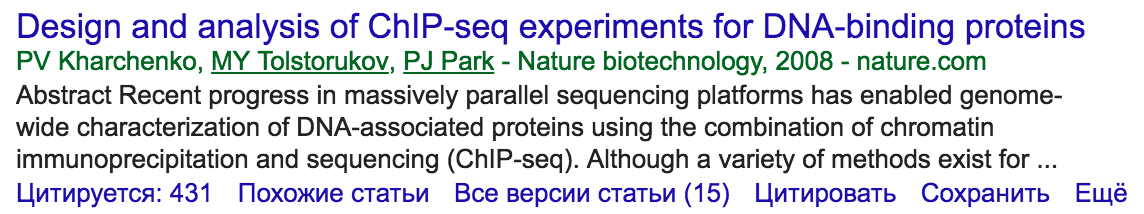
\includegraphics[width=\linewidth]{SPP.png}\\
SICER\\
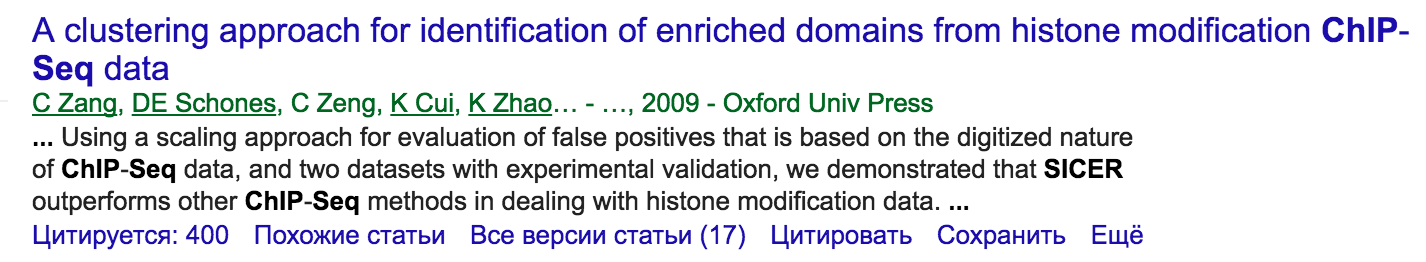
\includegraphics[width=\linewidth]{SICER.png}\\
CCAT\\
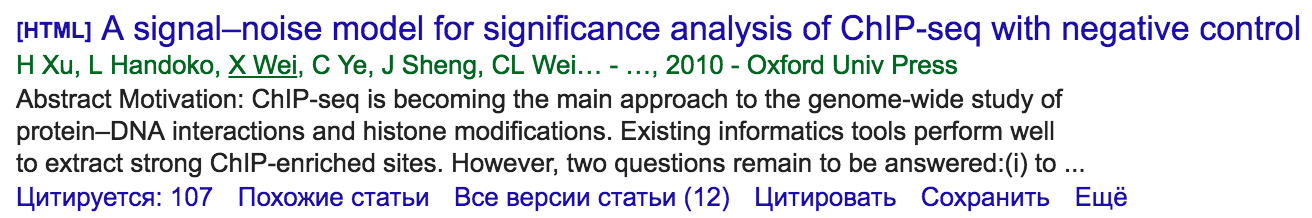
\includegraphics[width=\linewidth]{CCAT.png}\\
\end{frame}

\begin{frame}{Even less popular}
ZINBA\footnote{too slow \url{http://journals.plos.org/plosone/article?id=10.1371/journal.pone.0096303}}\\
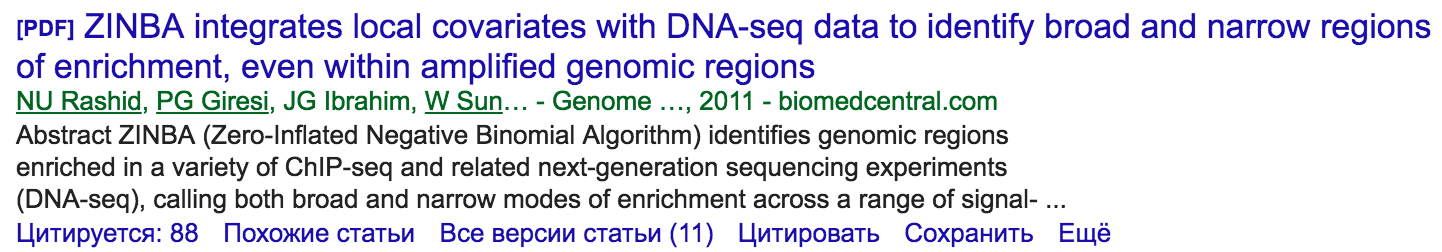
\includegraphics[width=\linewidth]{ZINBA.png}\\
RSEG\\
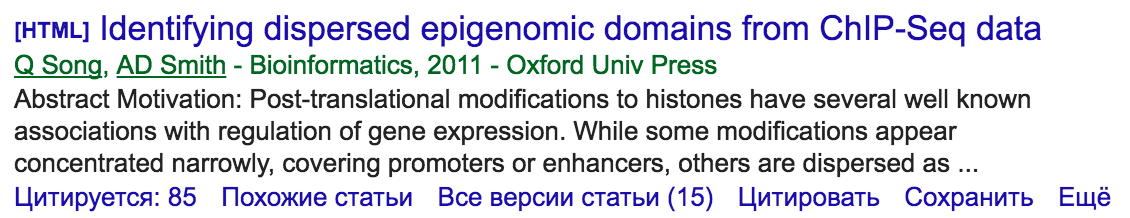
\includegraphics[width=\linewidth]{RSEG.png}\\
\end{frame}

\begin{frame}{Summary}
Consensus of 2 papers:
\begin{itemize}
\item Narrow peaks: MACS2 or SPP
\item Broad and mixed: SICER or ZINBA
\end{itemize}
TODO: test ZINBRA\footnote{\url{https://github.com/JetBrains-Research/zinbra}} in terms of IDR
\end{frame}

\begin{frame}{Mappability}


\end{frame}



\begin{frame}{Differential peak calling}
Two alternatives have been proposed.\footnote{Practical Guidelines for the Comprehensive Analysis of ChIP-seq Data}
\begin{itemize}
\item qualitative - hypothesis testing on multiple overlapping sets of peaks\footnote{\url{http://bioinformatics.oxfordjournals.org/content/28/24/3318.short}}.
\item quantitative -  proposes the analysis of differential binding between conditions based on the total counts of reads in peak regions or on the read densities, i.e., counts of reads overlapping at individual genomic positions\footnote{\url{http://www.biomedcentral.com/content/pdf/gb-2010-11-10-r106.pdf}}
\item model based
\end{itemize}
\end{frame}

\begin{frame}{Tools}
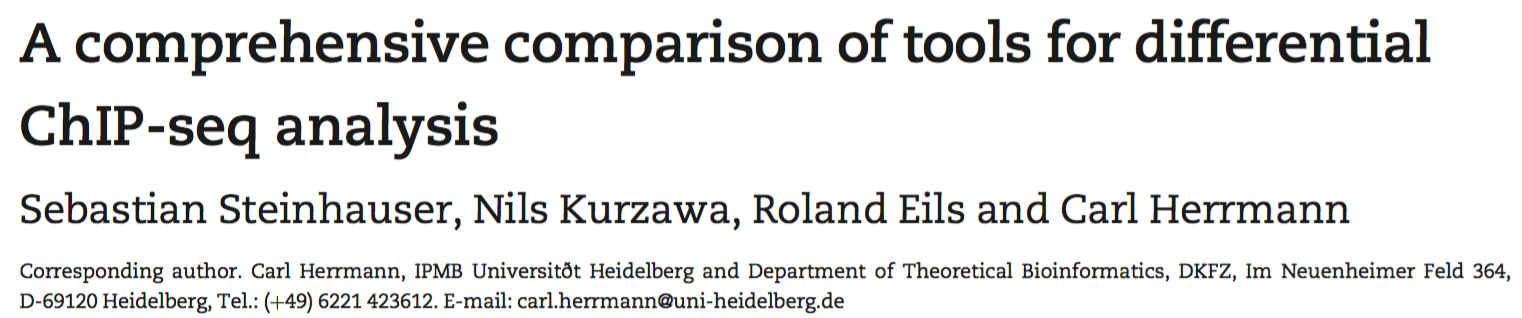
\includegraphics[width=\linewidth]{paperDPC.png}
\end{frame}

\begin{frame}{Problems}
\begin{itemize}
\item  Results obtained by different centers -  systematic bias correction required before data integration can be achieved
\item Reproducibility of the assays is often limited, especially in cases with additional constraints, for example low input material
\item ENCODE project showed that the amount of noise is >90\% (FRiP)
\item IDR for the rescue!
\end{itemize}
\end{frame}

\begin{frame}{Tools}
 Our criterion for tool selection was the availability of a working software that could be implemented without the need for extensive efforts for porting the code.\footnote{ChipDiff is not there}\\
 TODO: ZINBRA benchmark.
\end{frame}

\begin{frame}{Different aims - different approaches - different tools}
Tools
\begin{itemize}
\item Replicated or not
\item ChIPSeq or TF data
\item Control is required or not
\end{itemize}
\end{frame}

\begin{frame}{Test data}
NO gold standard for differential enrichment in ChIP signal.
\begin{itemize}
\item Each category is tested separately, 2 biological replicates for each condition\footnote{Replicates were pooled for single source tools}
\item TF: FoxA1 ChIP-seq for (E2)- and vehicle (Veh)-treated MCF7 (GSE59530) + expression data (GSE59531)
\item Shar ChIP-Seq: H3K27ac for hESC-H1 and mesenchymal stem cells (GSE16256)
\item Broad ChIP-Seq: H3K36me3 for myelome cells TKO vs NTKO (GSE57632)
\item Simulated datasets to estimate Sensitivity/Specificity
\item hg19, BWA, filter out duplicated/bad quality reads
\item MACS2 \\
narrow:  ‘-g hs -q 0.1 –call-summits’\\
broad: ‘-g hs -q 0.1 –broad’
\end{itemize}
\end{frame}

\begin{frame}{Params}
\begin{itemize}
\item NO silver bullet: NO common significant threshold. \\
When possible: FDR $\leq$ 0.01 or P-value $\leq$ 0.05.
\item Gene centric approach: ranked differential peaks by significance - select top 1000 closest genes\footnote{ChIPSeeker}
\item Functional annotation of regions $\pm$ 1.5kb around TSS\footnote{GREAT: single nearest gene}.
\item Jaccard index used as measure of differential peaks correspondence
\item Analyze single tool DR fraction in union of all DR from all tools
\end{itemize}
\end{frame}

\begin{frame}
\centering{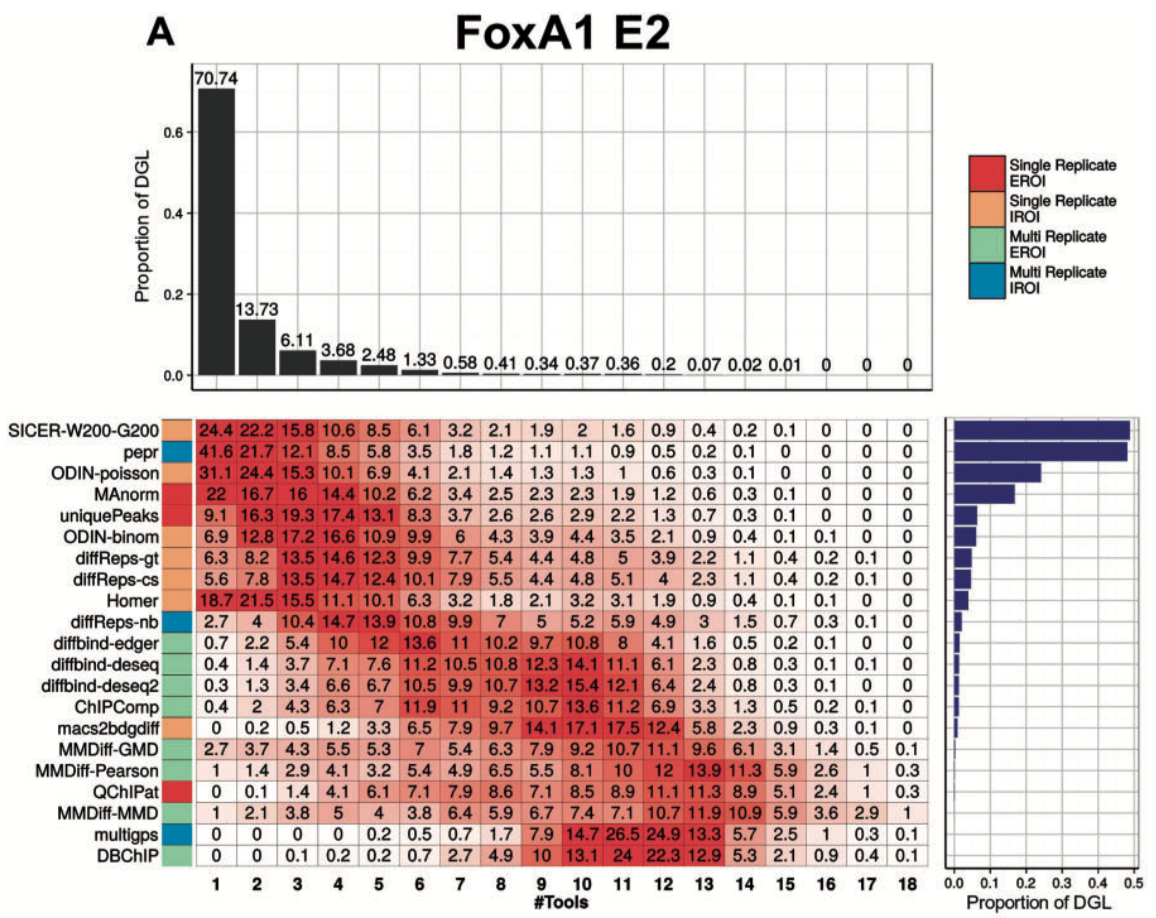
\includegraphics[width=0.9\linewidth]{foxa1.png}}\footnote{EROI/IROI-external regions required\\
Tools - DR is identified by number of tools}
\end{frame}

\begin{frame}
\centering{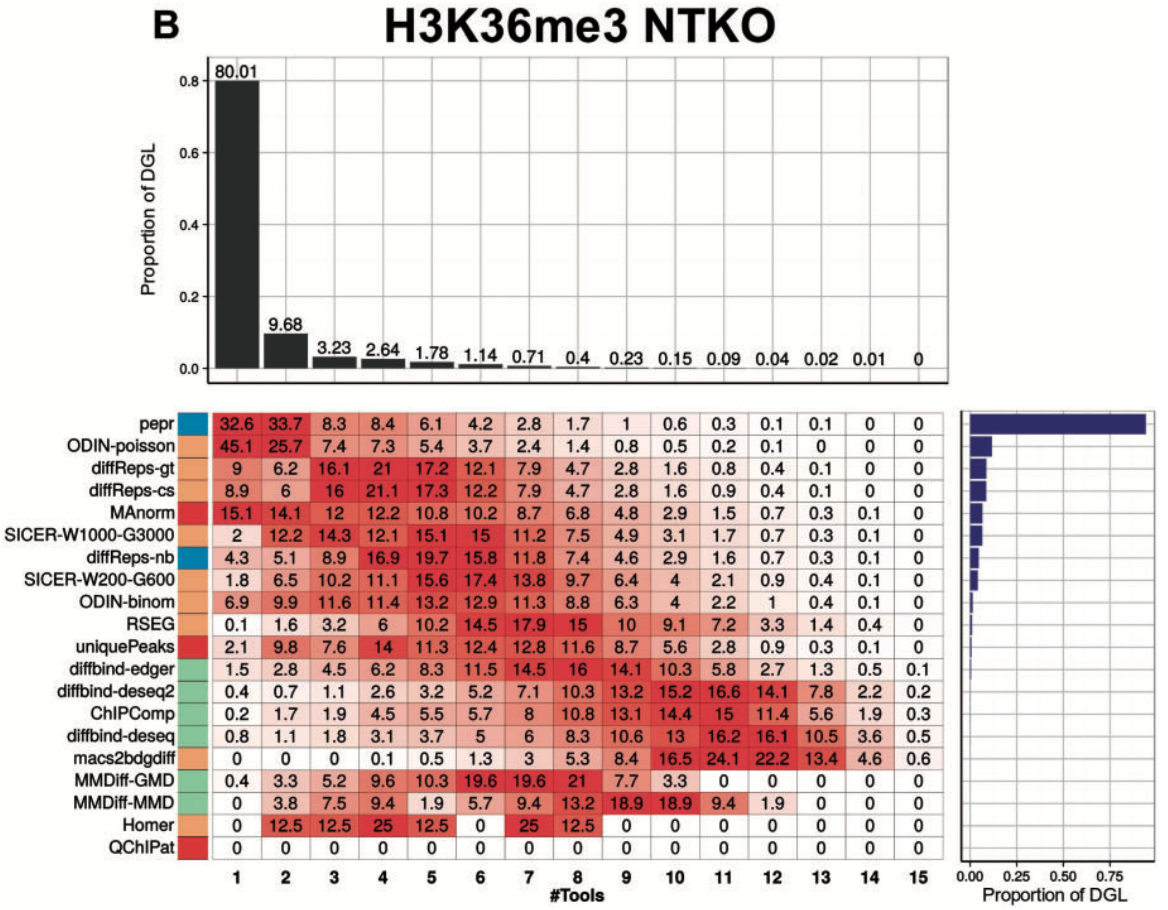
\includegraphics[width=0.9\linewidth]{h3k36me.png}}
\end{frame}

\begin{frame}{Results}
\begin{itemize}
\item Tools for differential ChIP-seq analysis show important differences in the number and size of detected differential regions (DR).
\item Methods taking into account replicates appear to be more robust than those handling single replicate data sets.
\item Inconsistent sets of DR will affect results based on sequence analysis, like detection of enriched transcription factor binding sites.
\item Analysis of functional enrichments based on neighboring genes appears to be more robust.
\item Some tools give good results with default parameters, like ChIPComp or diffBind when replicates are available, or MAnorm, Homer, macs2bdgdiff and RSEG with single replicates. The other tools would require more extensive fine-tuning of parameters to achieve satisfactory results.
\end{itemize}
\end{frame}

\begin{frame}{How do I choose?}
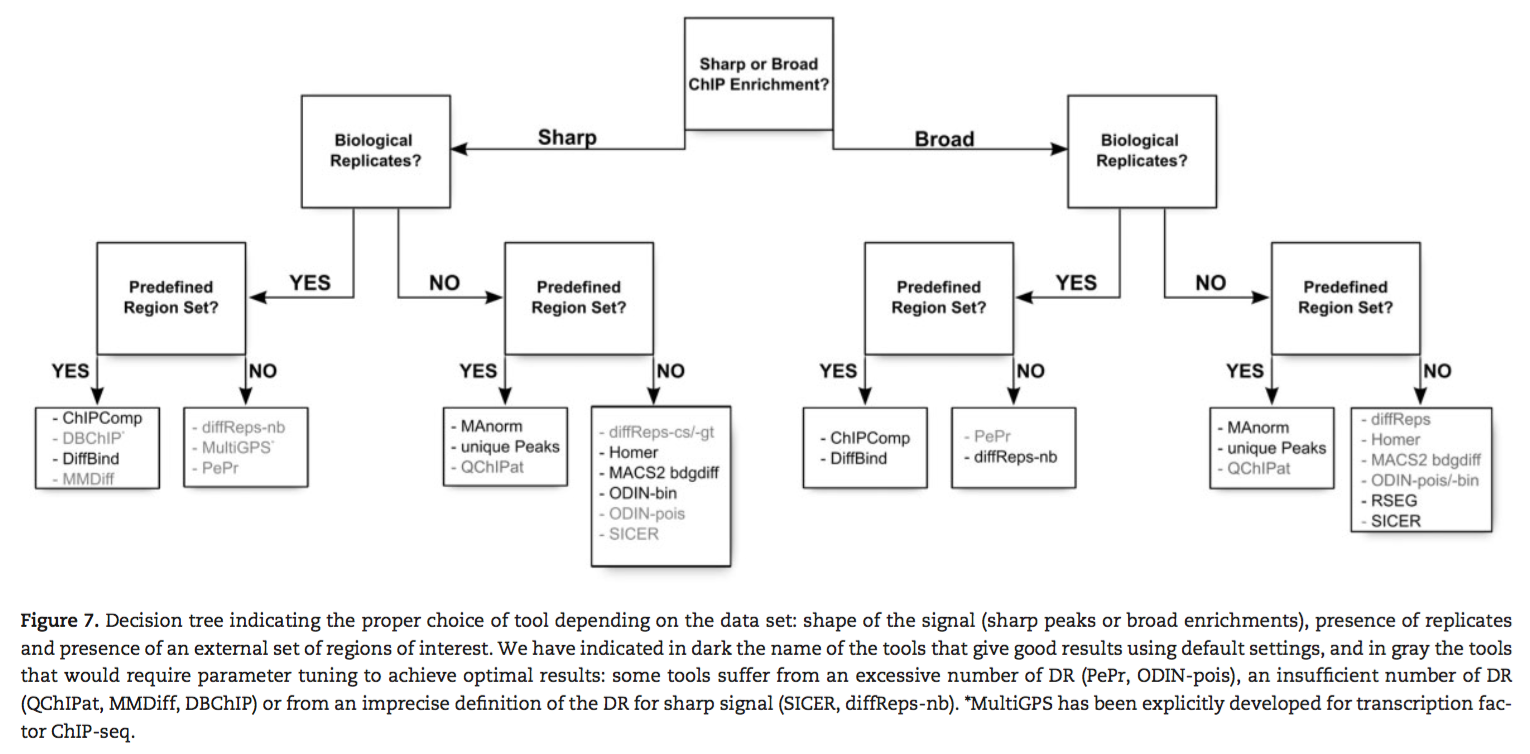
\includegraphics[width=\linewidth]{diffdt.png}
\end{frame}

\begin{frame}{Popular tools}
ChiPDiff\\
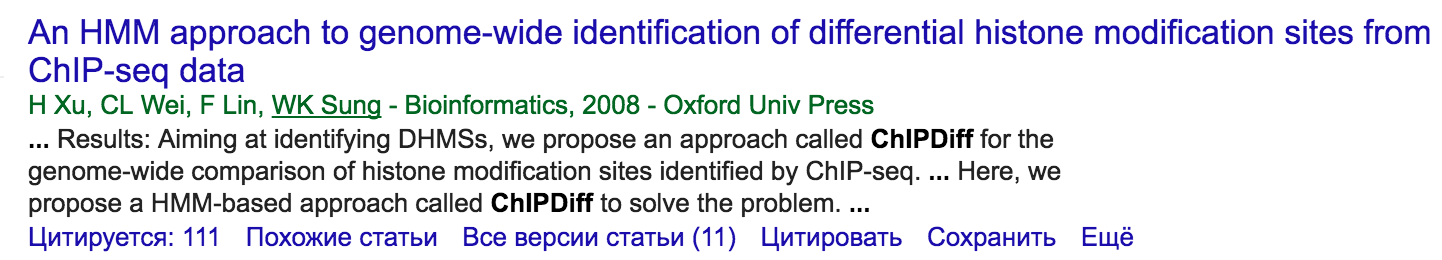
\includegraphics[width=\linewidth]{ChipDiff.png}\\
RSEG\\
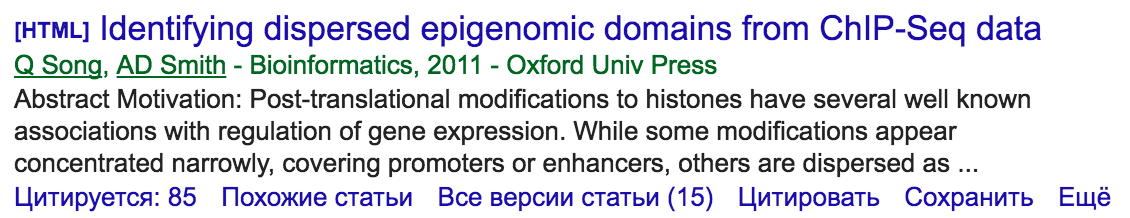
\includegraphics[width=\linewidth]{RSEG.png}\\
MAnorm\\
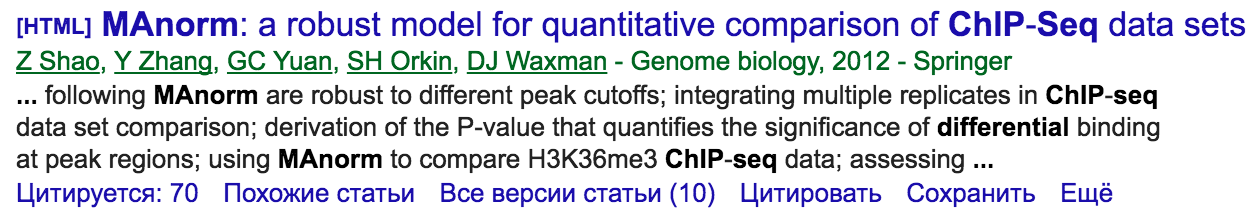
\includegraphics[width=\linewidth]{MAnorm.png}\\
\end{frame}

\begin{frame}{Less popular}
DiffBind\\

\includegraphics[width=\linewidth]{DiffBind.png}\\
ODIN\\
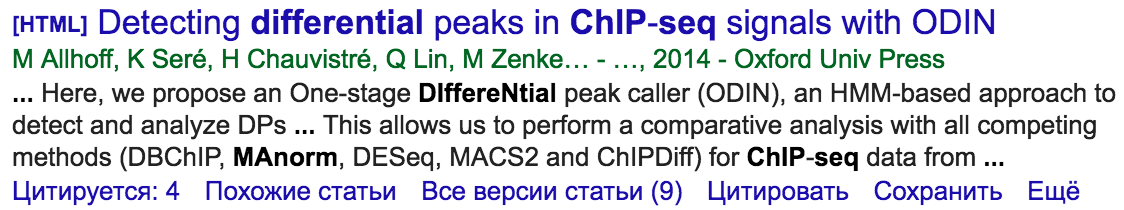
\includegraphics[width=\linewidth]{ODIN.png}\\
ChipComp\\
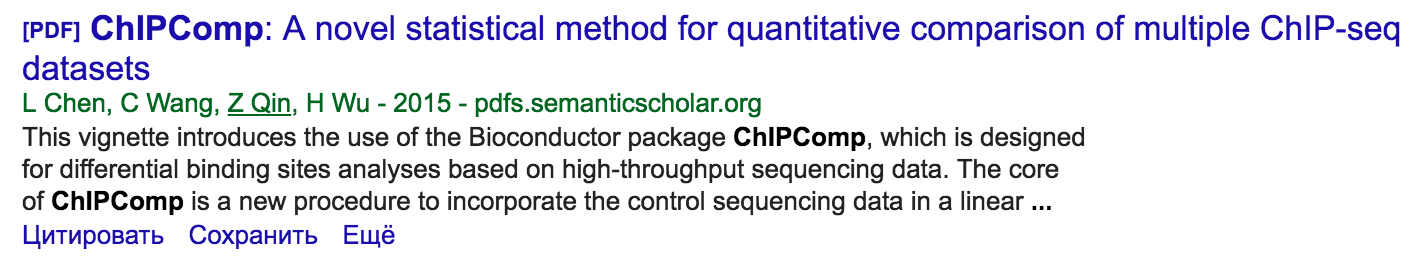
\includegraphics[width=\linewidth]{ChipComp.png}\\
\end{frame}

\begin{frame}
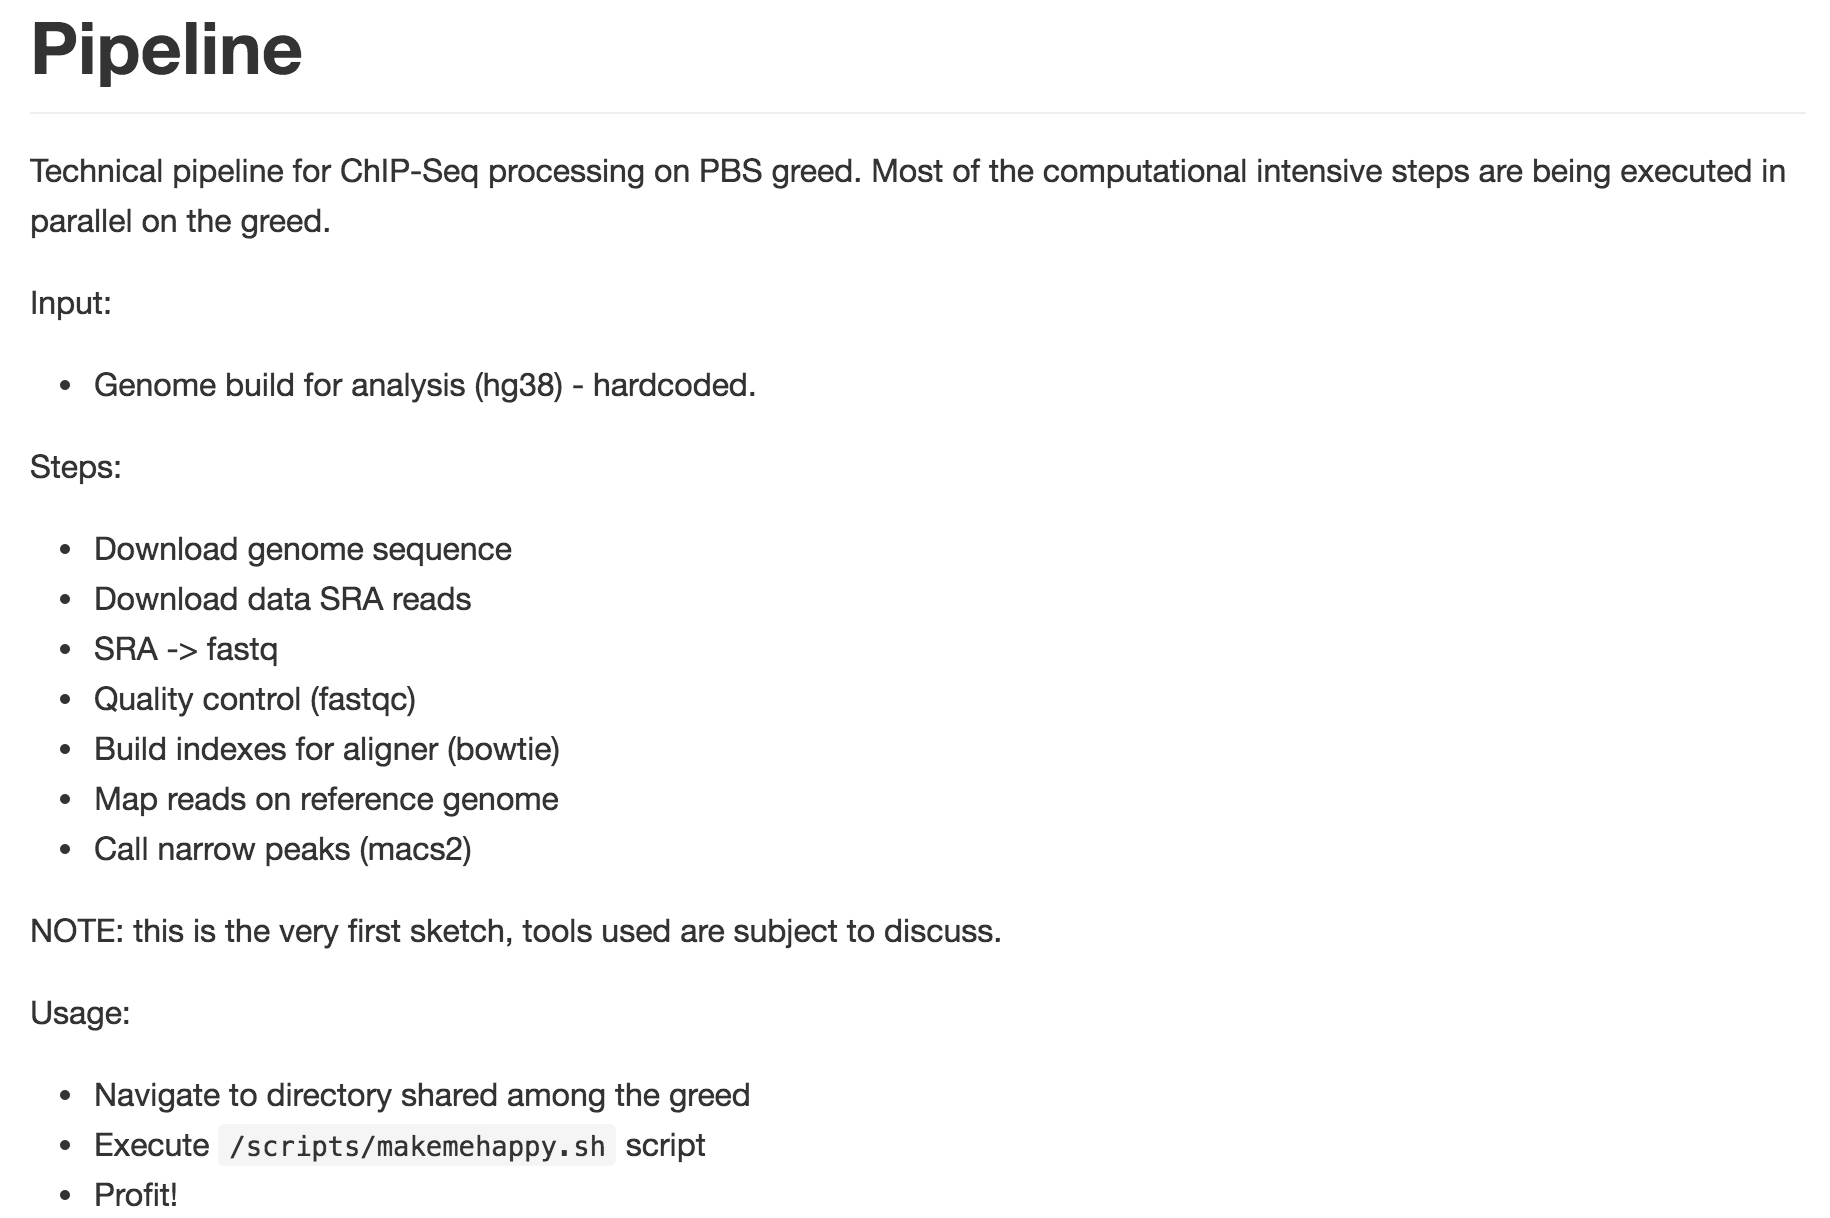
\includegraphics[width=\linewidth]{pipelinerepo.png}\footnote{\url{https://github.com/olegs/washu}}
\end{frame}

\begin{frame}{Some tech details}
\begin{itemize}
\item PBS computational greed
\item Shared /home/username and /scratch/username
\item Module system to "load" pre-installed software
\item Task are submitted and queued by qsub calls
\end{itemize}
\end{frame}

\begin{frame}{Pipeline executable}
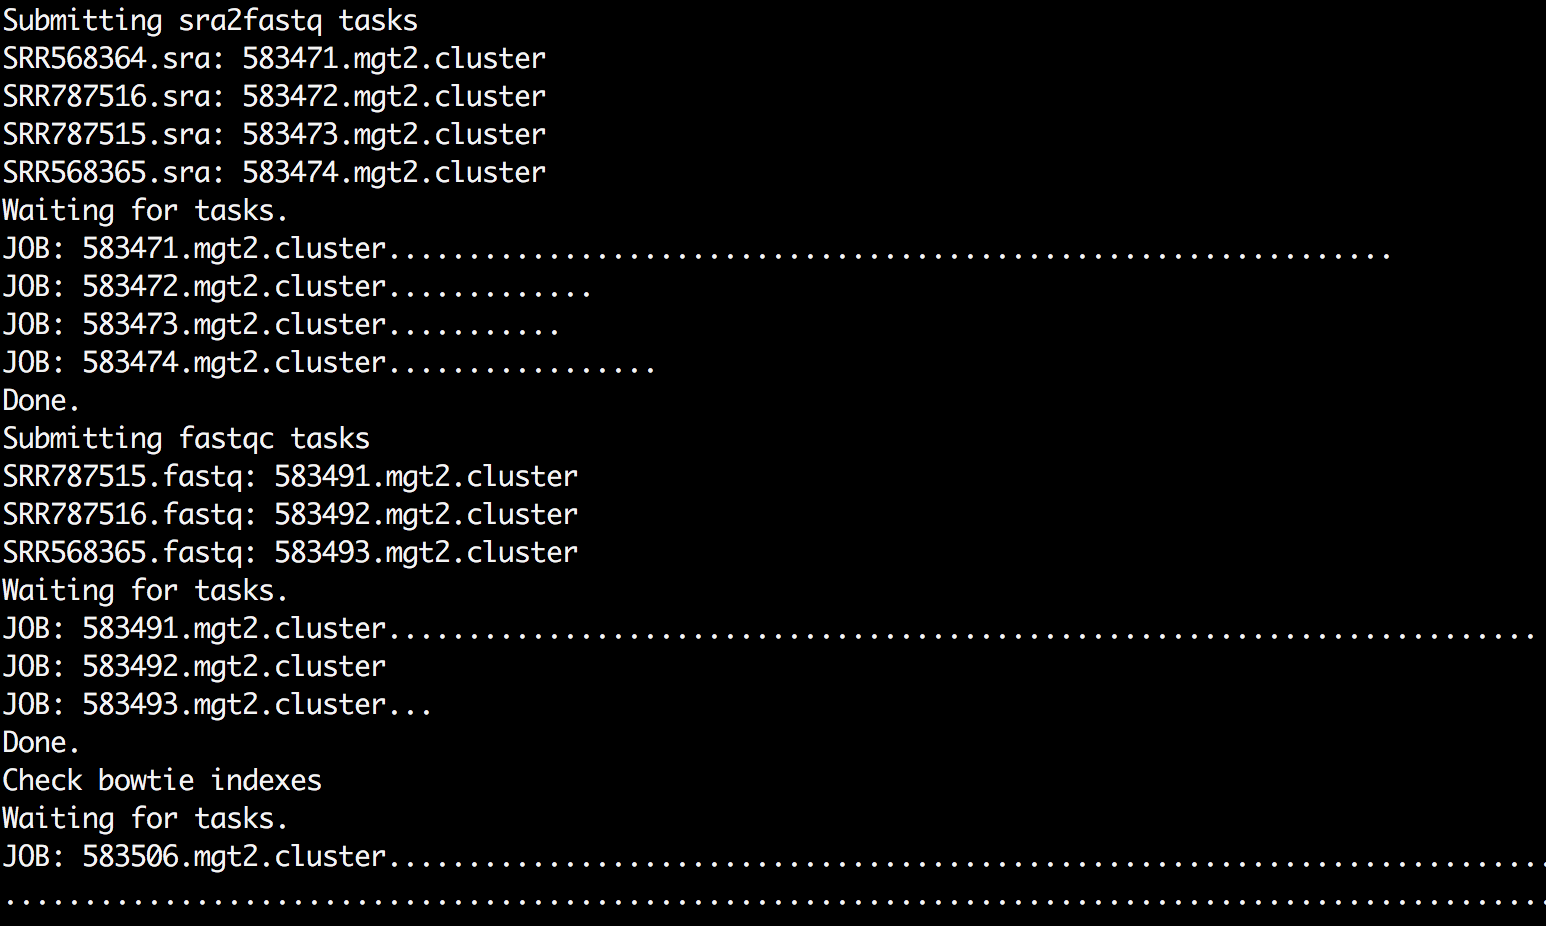
\includegraphics[width=\linewidth]{pipeline.png}\\
\end{frame}

\begin{frame}{Queues}
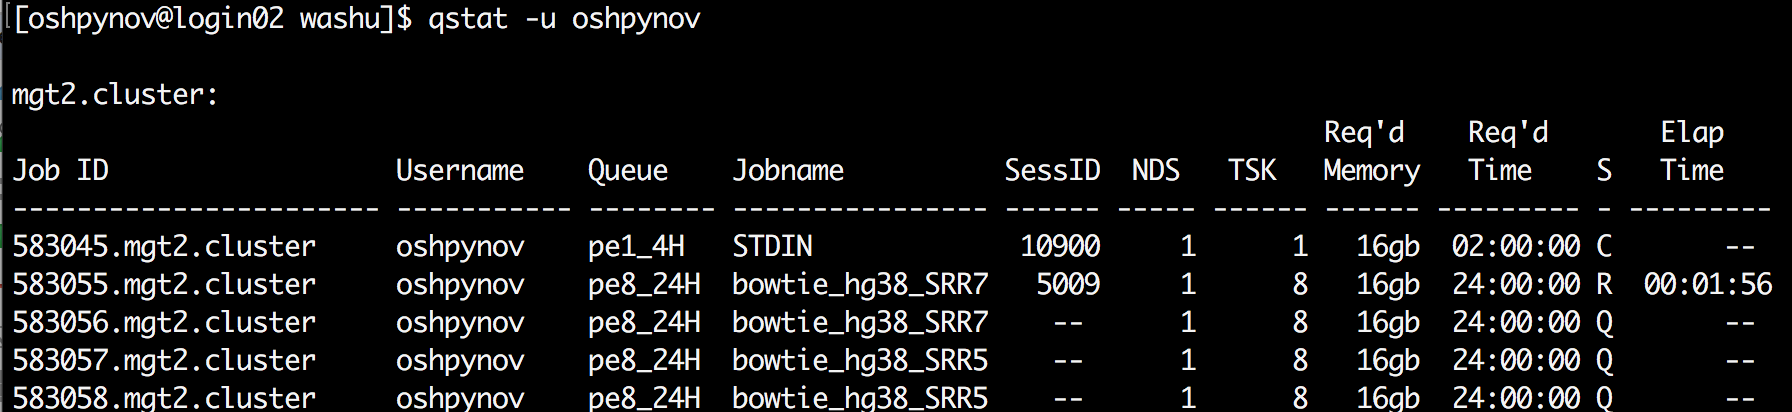
\includegraphics[width=\linewidth]{queue.png}\\
\end{frame}


\begin{frame}{Preliminary results}
Pipeline: \url{https://github.com/olegs/washu}
\begin{itemize}
\item Reads QC
\item Alignment stats
\item Lot's of things to do
\end{itemize}
\end{frame}


\begin{frame}
\centering{
	\huge{Thank you!}
}\\
\centering{
	@olegs\\
	oleg.shpynov@jetbrains.com\\
	\url{https://research.jetbrains.org/groups/biolabs}
}
\end{frame}

\end{document}
